\Chapter{フーリエ解析 超入門(大澤)}
\Section{はじめに}
本日は,数学科展示ますらぼにお越しくださり,また,本冊子$e^{\pi i}sode$を手に取ってくださり,誠にありがとうございます.

やっと数理科学研究科棟の空気に慣れ始めた私ですが,数学の世界というものは想像よりもはるかに広く,毎日が苦労の連続です.そんな日々だからこそ,今まで知らなかった世界が見えてくる,視界が広がっていく時の感動は一入です.

本冊子のテーマは「わたしのえぴそーど」ということで,私が高校生のときに初めて学んだフーリエ解析について少しだけ紹介したいと思います.私が初めて学んだ時の感動を多くの人と共有したいので,できるだけ平易な内容で(高校数学くらいを前提として),「こんな方法があるんだ」といったことを知って頂くような,そんな記事にするつもりです.

\Section{基礎知識}
高校1年生になると,いわゆる「サインコサイン」を学ぶと思います.高校の数学と言えば「サインコサイン」と「ビブンセキブン」というのが,語呂の良さなどもあって数学が苦手な学生の敵にされがちです.

高校2年生で,関数$\sin x$と$\cos x$を学びます.直角三角形から生み出された「サインコサイン」を拡張した概念です.ご存じ,周期$2 \pi$で1と-1の間をウロウロ振動する関数です.

$\sin 2x,\sin 3x,\dotsc$ を考えると,これはだんだん周期が短くなります. $2\sin x,3\sin x,\dotsc$ を考えると,振動の振幅がだんだん大きくなります.
これらの関数について微分・積分を考えることが出来ます.また,これらの関数を掛け合わせて積分したものについて,以下の関係式が成り立ちます.
\begin{alignat*}{2}
  \int_{-\pi}^\pi \sin mx \sin nx dx &= 0
  & \qquad &
\text{($m$, $n$ は整数,$m \neq n$)} \\
\int_{-\pi}^\pi \sin mx \sin nx dx &= \pi
& &
\text{($m$, $n$ は整数,$m = n$)}
\end{alignat*}

つまり,$\sin x$の関数の周期のなかで,振動の回数が違う二つのサイン関数を掛け合わせて積分すると0になり,同じ振動数の関数どうしを掛け合わせると$\pi$になります.この積分は,加法定理から導かれる
$\sin x \sin y = \frac{1}{2} (\cos(x-y)-\cos(x+y))$
から計算できます.

$\cos x$についても同じ関係式が成り立ちます.
さらに,$\sin x$と$\cos x$を掛け合わせて積分すると, $m$ と $n$ が整数なら同じ値でも違う値でも,
\[
  \int_{-\pi}^\pi \sin mx \cos nx dx = 0
\]
が成り立ちます.

\Section{フーリエ級数}
以上の前提を踏まえてフーリエ級数を定義します.

フーリエ級数はざっくり言うと,「『まともな』関数ならば,無限個の三角関数の足し合わせで表現できる」といった考え方です.数式で表現すると以下のようになります.

\[
  f(x) = \sum_{n=1}^\infty (a_n \cos nx + b_n \sin nx + C)
\]

さらっと一つの式でまとめましたが,これは大層なことを言っていて,つまり直線でも放物線でも,どんな関数でもサインとコサインを足し合わせ続ければ再現できるということなのです!

『まともな』関数と言いましたが,例えば有理数に対して1を,無理数に対して0を返すような関数はこのような展開が出来ません.最低限の条件として,関数が区部的$C^1$級,つまりはいくつかの点で関数を区切った時にそれぞれのパーツが微分可能であれば構いません.高校までで習うほとんどの関数なら大丈夫なのです.\\

さて,本当に表されるのであれば,各係数$a_n,b_n,C$は先程の積分の結果を使えば簡単に求められます.
$k$を整数として,両辺に$\cos kx$をかけて積分します.
\[
  \int_{-\pi}^\pi f(x) \cos kx = \sum_{n=1}^\infty (a_n \cos nx \cos kx+ b_n \sin nx \cos kx + C \cos kx)
\]
そうすると,右辺は$\cos kx \cos kx$の積分だけが1となって残り,残りは先程の計算で0になってしまいます.$\sin nx \cos kx$の積分も消えて,$\cos kx$の積分も一周期分の積分のため消えてしまいます.したがって,
\[
  \frac{1}{\pi} \int_{-\pi}^\pi f(x) \cos kx dx = a_k
\]
が出てきて,すべての $n$ について係数(フーリエ係数)がわかります.
また,$\sin kx$をかけたり,そのまま積分することで,
\[
  \frac{1}{\pi} \int_{-\pi}^\pi f(x) \sin kx dx = b_k
\]
\[
  \frac{1}{2 \pi} \int_{-\pi}^\pi f(x) dx = C = \frac{a_0}{2}
\]
が導かれます.

また,オイラーの公式
\[e^{ix} = \cos x + i \sin x\]
を用いると,フーリエ級数は以下のように簡単に書き換えることもできます.

\[
  f(x) = \sum_{n=-\infty}^\infty c_n e^{inx}
\]

\[
  c_n = \frac{1}{2\pi} \int_{-\pi}^\pi f(x) e^{-inx} dx
\]

\Section{フーリエ級数の収束}
とりあえず,級数が収束するなら$a_n,b_n,C$が決定することは分かりました.問題は本当に収束するのかどうかです.

数学が得意な人にとってはここが一番気になるところだと思いますが,誌面の都合上,証明の流れだけお話しようと思います.\\

$f$ の定義域の点 $x$ において,右側から近づけた極限$f(x+0)$と,左側から近づけた極限$f(x-0)$について考えます.また,
\[
  S_N[f](x) = \sum_{n=-N}^N c_n e^{inx}
\]
とおきます.これはフーリエ級数の足し合わせを $N$ 番目まで行ったものです.

$I_N = S_N[f](x) - \frac{1}{2}(f(x+0)+f(x-0))$とおき,
\[
  \lim_{N \to \infty} I_N = 0
\]
を示せば, $f$ が $x$ で連続ならば $f$ をフーリエ級数展開したときに収束してくれることが示せます.

ここで,$I_N$を分解します.分解のために以下の関数を定義します.
\[D_N(x) = \frac{\sin(N + \frac{1}{2})x}{\sin(\frac{x}{2})}\]
これをディリクレ核と呼びます.これを用いると,$I_N$を分解して,
\[
  I_N = (\frac{1}{2\pi} \int_{-\pi}^0 f(x+t) D_N(t) dt - \frac{1}{2} f(x-0)) +  (\frac{1}{2\pi} \int_0^\pi f(x+t) D_N(t) dt - \frac{1}{2} f(x+0))
\]
とできます.あとは前半部と後半部がそれぞれ収束することを示せばよいです.

尻切れトンボになってしまい申し訳ありませんがここまでにします.本当は$D_N(x)$の性質からディリクレ核の積分などを補題として使い,これらが収束することを示すのですが,興味がある人は是非調べてみてください,と言いつつ丸投げします.

\Section{私が高校生だったころのフーリエ級数}
いま求めたフーリエ級数ですが,何に使えるのか,という疑問は当然出てきます.

ひとつとしては,すべての関数が基本となる波の足し合わせと言っているのだから,例えば任意の種類の音を基本となる音だけ用いて再現することが可能になります.さらに熱方程式の解の導出にも表れ,物理や工学の世界で大きく発展できそうです.

しかし,当時この手法を知ったころの私が惹かれたのは,むしろ副産物の方でした.

いま,$f(x) = x^2$ としてフーリエ級数を計算します.この時,この関数を$({-\pi} \leq x \leq \pi)$に制限し,$(x \leq -\pi)$や$(x \geq \pi)$同じ${2\pi}$周期で何度も同じ放物線が現れるようにします.

\begin{figure}[h]
  \begin{center}
    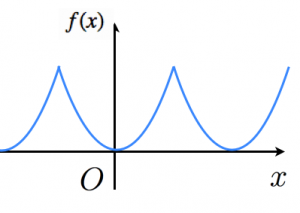
\includegraphics[clip,width=7.0cm]{osawa.png}
    \caption{放物線(周期$2\pi$)}
    \label{f_para}
  \end{center}
\end{figure}

フーリエ係数を求めると,
\[
  \frac{a_0}{2} = \frac{1}{\pi} \int_{-\pi}^\pi x^2 dx = \frac{\pi^2}{3}
\]
\[
  a_n = \frac{1}{\pi} \int_{-\pi}^\pi x^2 \cos nx dx = (-1)^n \frac{4}{n^2}
\]

また, $f$ は偶関数( $y$ 軸について対称)である.$\cos nx$は同様に偶関数なので足し合わせても差し支えは無いが,$\sin nx$を足し合わせてしまうと,これは奇関数なので,足し合わせてしまうと結果が偶関数でなくなってしまう.
したがって,$b_n = 0$が成り立つ.

つまり,
\[
  f(x) = x^2 = \frac{\pi^2}{3} + \sum_{n=1}^\infty (-1)^n \frac{4}{n^2} \cos nx
\]

ここで,$x = \pi$を代入すると,
\[
  \pi^2 = \frac{\pi^2}{3} + \sum_{n=1}^\infty \frac{4}{n^2}
\]
が成り立ち,整理すると
\[
  \sum_{n=1}^\infty \frac{1}{n^2} = \frac{\pi^2}{6}
\]
となります.これは,自然数の2乗の逆数を足し合わせた時の極限になります.\\

無限級数の和として,無限等比級数は高校数学の範囲で求められますが,$\sum_{n=1}^\infty \frac{1}{n^2}$については求められませんでした.しかしフーリエ級数を使えば,副産物としてこのような極限が求められるのです.

さらに別の関数を使えばこのような極限も求められます.
\[
  \sum_{n=1}^\infty \frac{1}{n^4} = \frac{\pi^4}{90}
\]
\[
  \sum_{n=1}^\infty \frac{1}{n^6} = \frac{\pi^6}{945}
\]

この,$\sum_{n=1}^\infty \frac{1}{n^p} = \zeta(p)$はゼータ関数といい,複素数に拡張することが出来ます.ゼータ関数の零点についての主張が,かの有名なリーマン予想というわけです.\\


\Section{フーリエ変換}
先のフーリエ級数では周期$2\pi$の関数を扱いましたが,世の中の関数の周期は$2\pi$だけとはいきません.さらに周期$L$の関数を考え,$L$が無限大のときを考えれば,周期関数以外でもこの手法が役に立ちそうです.

周期$2L$の関数のフーリエ級数は,変数変換などを使って以下のように表されます.
\[
  f(x) = \sum_{n=-\infty}^\infty c_{L,n}(f) e^{inx\pi/L}
\]
\[
  c_{L,n} = \frac{1}{2L} \int_{-L}^L f(y) e^{-iny\pi/L} dy
\]
ここで,$\Delta\xi = \frac{\pi}{L},{\xi_k} = \frac{k\pi}{L}$とおきます.
\[
  f(x) = \sum_{n=-\infty}^\infty c_{L,n}(f) e^{i{\xi_k}x} \frac{\Delta\xi}{\Delta\xi}
  =\frac{1}{2\pi} \sum_{n=-\infty}^\infty 2{L}(\frac{1}{2L} \int_{-L}^L f(y) e^{-i{\xi_k}y} dy) e^{i{\xi_k}x} {\Delta\xi}
\]
ここで,$L \to \infty$のときを考えると,${\Delta\xi} \to 0$になるが,このときリーマン積分の定義より総和が積分に置きかわります.
\[
  f(x) = \frac{1}{2\pi} \int_{-\infty}^\infty (\int_{-\infty}^\infty f(y) e^{-i\xi y}dy) e^{i\xi x}d\xi
\]

2つの積分操作が為されていますが,それぞれを関数の変換とみなして以下のように表現します.

\[
  \mathcal{F}[f](\xi) = \int_{-\infty}^\infty e^{-ix\xi} f(x) dx
\]
\[
  \mathcal{F}^{-1}[f](x) = \frac{1}{2\pi} \int_{-\infty}^\infty e^{ix\xi} f(\xi) d\xi
\]

上をフーリエ変換,下をフーリエ逆変換といいます.フーリエ級数を拡張した時の式から,フーリエ変換をしたあとにフーリエ逆変換をすると元の関数に戻ることがわかります.\\
フーリエ変換の面白いところは色々ありますが,例えば元の関数に微分操作,積分操作を行うとフーリエ変換は以下のように書き換わります.\\
\[
  \mathcal{F}[\frac{df(x)}{dx}](\xi) = i\xi \mathcal{F}[f](\xi)
\]
\[
  \mathcal{F}[\int_{-\infty}^x f(y) dy](\xi) =\frac{1}{i\xi} \mathcal{F}[f](\xi)
\]
これは,例えば微分方程式や積分方程式を解くときに,フーリエ変換をして微分操作や積分操作を掛け算に直してから計算し,フーリエ逆変換で戻せば解が求められることを意味しています.このフーリエ変換や,ラプラス変換と呼ばれる別の変換は,このように関数に対する操作を簡単にしてくれます.こうしてフーリエ級数を発展させて,関数の変換を導出しました.

\Section{おわりに}
以上,フーリエ級数とフーリエ変換について簡単にですが紹介しました.

これらフーリエ解析については,東大の数学科では3年の秋〜冬に学習します.フーリエ変換は工学の世界で頻繁に出てくるので,工学部では数学科より早く学ぶのですが,数学科ではルベーグ積分の基礎をきちんと学習してからフーリエ解析に入り,収束の証明をきちんと行います.

この冊子の中では比較的平易な内容ではありますが,私が出会ったときに一番好奇心を掻き立てられたのがこの単元だったので,「わたしのえぴそーど」というタイトルにふさわしいと思い紹介しました.

ぜひ「ますらぼ」で,それから今後もいろいろな機会で,数学の世界に触れていただければと思います.
\begin{thebibliography}{9}
\item 新井 仁之 「新・フーリエ解析と関数解析学」 培風館
\item 竹内 淳 「高校数学でわかるフーリエ変換」 講談社ブルーバックス
\end{thebibliography}

文責:大澤 哲史
